\documentclass[a4paper,12pt]{article}
\usepackage{graphicx} 			% Para insertar imagenes
\usepackage{indentfirst} 	% Para sangrar párrafos después de secciones
\setlength{\parindent}{1.5cm} 	% Sangría de 1.5 cm
\usepackage{minted} 	% Para insertar código 
\usepackage{float}
\usepackage[spanish, es-tabla]{babel}
\usepackage{tcolorbox} % Para secciones en destacado
\usepackage{amsmath}
\usepackage{amssymb}
\usepackage[hidelinks]{hyperref} % Para enlaces

\title{Práctica 2 parte 2: Calculadora con Apache Thrift }
\author{Ángel Rodríguez Faya}
\date{26 de marzo de 2026}

\begin{document}
	
	% --- PÁGINA 1: LA PORTADA ---
	\begin{titlepage}
		\centering
		\vspace*{1cm}
		
		{\huge\bfseries Práctica 2 parte 2: Calculadora con Apache Thrift \par}
		\vspace{1 cm}
		
		{\Large Desarrollo de Sistemas Distribuidos. Grupo DSD-3. \par}
		\vspace{0.25cm}
		{\Large Grado en Ingeniería Informática \par}
		\vspace{0.25cm}
		{\Large Curso 2025-2026.\par}
		\vspace{0.25cm}
		{\Large ETSIIT. Universidad de Granada.\par}
		\vspace{1 cm}
		
		\noindent % Evita la sangría para que aproveche todo el ancho
		\begin{minipage}[c]{0.55\textwidth}
			% La imagen ocupa el 100% del ancho DE ESTA CAJA (no de la hoja)
			
\includegraphics[width=\linewidth]{./imagenes_necesarias/Logotipo_ETSIIT_Horizontal_color.png}
		\end{minipage}% <--- Este % es importante para que no añada espacios extra
		\hfill % Rellena el espacio en medio empujando las cajas a los extremos
		\begin{minipage}[c]{0.40\textwidth}
			\raggedleft % Alinea esta imagen a la derecha dentro de su caja
			
\includegraphics[width=\linewidth]{./imagenes_necesarias/UGR-LOGO-color.png}
		\end{minipage}
		
		\vspace{0.5 cm}
		
		{\large\bfseries Autor: \par}
		{\large Ángel Rodríguez Faya \par}
		\vspace{0.5cm}
		
		{\large\bfseries Profesor: \par}
		{\large José Ángel Segura Muros \par}
		\vspace{1 cm}
		
		{\large\bfseries Fecha de entrega: \par}
		{\large 27 de marzo de 2026\par}
		
	\end{titlepage}
	% El entorno 'titlepage' hace el salto de página automáticamente al cerrar.
	
	% --- PÁGINA 2: EL ÍNDICE ---
	\tableofcontents
	\newpage % <--- Fuerza el salto a la página 3
	
	% --- RESTO DE PÁGINAS:
	\section{Introducción.}
		En esta práctica tenemos que volver a implementar la calculadora de la 1ª parte de la práctica 2, que realizaba 4 operaciones básicas (suma, resta, multiplicación y división) más 3 operaciones para calcular áreas de tres figuras geométricas. Pero, en este caso, en lugar de implementarlo con \texttt{Sun RPC} tenemos que hacerlo con \texttt{Apache Thrift}.
		
		\texttt{Apache Thrift} es un \textit{framework} de desarrollo de software de código abierto, creado originalmente por Facebook y gestionado por la \textit{Apache Software Foundation}, que permite la comunicación eficiente y directa entre servicios escritos en diferentes lenguajes de programación. Además tiene un motor de generación de código para crear servicios \textbf{RPC} \textit{(Remote Procedure Call)} que funcionan de manera eficiente y sin problemas entre C++, Java, Python, etc., facilitando así el desarrollo de sistemas distribuidos. Para más información, podemos visitar la  \href{https://thrift.apache.org/}{\underline{página web oficial de Apache Thrift}}.
		
	\section{Requerimientos.}
		El propósito de este apartado es detallar los requisitos (tanto básicos como avanzados) que se nos pedían para realizar la práctica, además de hacer más comprensible el documento, ya que de un simple vistazo se puede ver lo que se implementa o lo que no este proyecto de la calculadora distribuida.
	
		\subsection{Requerimientos básicos.}
			Como requisitos básicos se nos pedía que realizara las 4 operaciones básicas descritas en la 1ª parte de la práctica, además de añadir el cálculo del área de cuadrados, triángulos y círculos. Estas operaciones \textbf{se encuentran implementadas y disponibles.}

		\subsection{Requerimientos avanzados.}	
			Como requerimientos avanzados que se nos proporcionaban de ejemplo para añadir funcionalidades a nuestra calculadora se encuentran:
			
			\begin{itemize}
				\item \textbf{Enviar una estructura de operaciones y operandos para que se realicen a la vez.} Más adelante, en el apartado de componentes podremos ver que hay definida una estructura llamada \texttt{Operación} que encapsula los dos operandos y el operador para realizar la correspondiente operación, aunque también se tiene en cuenta que hay operaciones que sólo necesitan un operador. En el menú de la calculadora lo veremos implementado como \textbf{Procesar un lote de operaciones}, al que se le pasa una colección de objetos de la estructura \texttt{Operación}, calcula el resultado de cada uno de ellos, y luego nos devuelve todos los resultados a la vez.
				
				\item \textbf{Operaciones con  matrices.} Se puede realizar la \textbf{suma} y \textbf{multiplicación} de dos matrices, que se piden al usuario por la terminal. No hay implementadas operaciones con vectores como tal, pero el motivo era por simplificar y no sobrecargar tanto el menú. \textbf{Aunque se pueden realizar operaciones con vectores manteniendo una de las componentes fijas} (por ejemplo, para sumar dos vectores de \textit{n elementos}, introducimos dos matrices de dimensiones \textit{1 x n}, es decir, tienen 1 sola fila y \textit{n} columnas).
				
				\item \textbf{Gestión de excepciones}. Se ha tenido en cuenta a la hora de implementar las operaciones ya que si se produce una excepción, bien porque estamos introduciendo un valor incorrecto (por ejemplo un carácter donde pide un número), o bien porque no hemos podido establecer una conexión con el servidor; todas ellas se han tratado de capturar y manejar para que, en lugar de que nuestro programa finalice de forma repentina y no sepamos porque, muestre donde ha ocurrido la excepción y sepamos reconocer de donde viene el problema. Además, en el fichero \texttt{calculadora.thrift} donde definimos los tipos de datos y los servicios, también se ha definido una excepción para que se lance cuando se intenta realizar una operación que no es posible (como por ejemplo dividir entre 0 o calcular el logaritmo de un número negativo).
				
				\item \textbf{Utilizar distintos lenguajes para crear el cliente y/o el servidor.} En mi caso, he implementado el cliente en Python y el servidor en Java y en Python. El objetivo de esto es tratar de aprender y también demostrar que no hace falta que el cliente y el servidor estén escrito en el mismo lenguaje, si no que puede estarlo en diferentes lenguajes e igualmente pueden trabajar juntos gracias a herramientas como \texttt{Apache Thrift} que hacen que esto sea posible.
				
				\item \textbf{Cualquier otra operación que se considere interesante.} Además de las operaciones ya mencionadas anteriormente, se han añadido las siguientes:
				
				\begin{itemize}
					\item Potencia de x elevado a y.
					\item Raíz cuadrada de x.
					\item Logaritmo en base 10 de x.
					\item Logaritmo neperiano (o natural) de x.
					\item Seno de x grados
					\item Coseno de x grados
					\item Tangente de x grados.
					\item Además, exceptuando las matrices que trabajan con números enteros, el resto de operaciones de la calculadora se realizan con números en coma flotante (también llamados \texttt{double} o \texttt{float} dependiendo del lenguaje de programación.)
				\end{itemize}
				
			\end{itemize}
		
	\section{Componentes.}
		En esta sección veremos cada uno de los componentes que forman este programa/práctica. 
		
		Además, en la siguiente imagen podemos ver el diagrama de clases en UML. También se encuentra disponible en formato \texttt{.png} en \newline \texttt{memoria/imagenes\_necesarias/diagrama\_de\_clases.png}
		
		\begin{figure}[H]
			\centering
			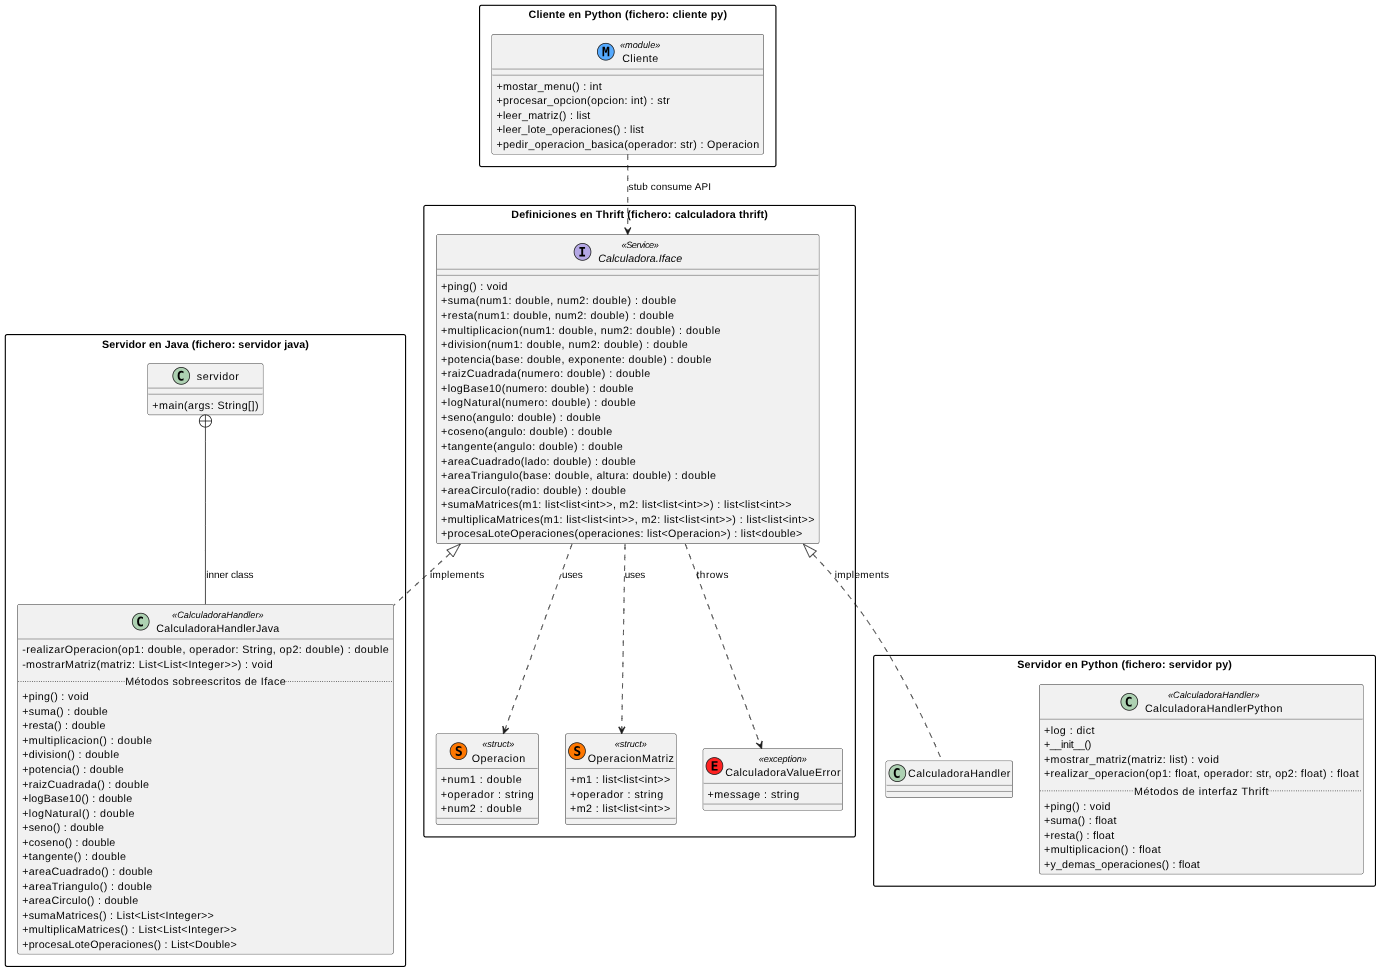
\includegraphics[width=1\linewidth]{./imagenes_necesarias/diagrama_de_clases.png}
			\caption{Diagrama de clases.}
			\label{fig:dc_p2_parte2}
		\end{figure}
		
		\subsection{Calculadora en Apache Thrift.}
			Es el fichero \textbf{IDL} (\textit{Interface Definition Language}). Se encuentra en el archivo \texttt{calculadora.thrift} y su contenido es:
			
			\inputminted[linenos, frame=lines, fontsize=\footnotesize]{Thrift}{../codigo/calculadora.thrift}
			
			 El archivo \texttt{calculadora.thrift} podríamos definirlo como el \textbf{\textit{contrato de comunicación}} que firman las partes implicadas en nuestro sistema distribuido, el cliente (que recordamos que estaba implementado en Python) y el servidor (implementado tanto en Python como en Java). En él se establece tres cosas: qué se puede hacer, cómo se puede hacer o cómo se debe pedir y qué vamos a recibir, sin importarle el lenguaje de programación en el que se vaya a desarrollar después. Es por eso que tenemos el cliente y el lenguaje implementados en diferentes lenguajes de programación.
			 
			 Vamos a distingir 4 partes importantes dentro de nuestro archivo \newline \texttt{calculadora.thrift}:
			 \begin{itemize}
			 	\item \textbf{Espacios de nombres (\textit{Namespaces})}. Le dicen al compilador de Thrift cómo debe organizar el código cuando lo traduzca. En nuestro archivo tenemos \mintinline{Thrift}|namespace java calculadora| que es necesario para poder generar el código en Java. En este caso, se le indica al compilador que meta el código de Java en un paquete llamado "\texttt{calculadora}".
			 	
			 	\item \textbf{Excepciones especializadas \textit{(Exceptions)}}. Nos permiten crear errores a medida tal que, si el servidor detecta que no es posible realizar una operación (por ejemplo, dividir entre cero), le envía este error o excepción al cliente y este ya sabe que se trata de un error producido por la imposibilidad de realizar una acción. En nuestro código, la excepción personalizada es \mintinline{Thrift}|except CalculadoraValueError|.También existen otras opciones predefinidas en los lenguajes de programación.
			 	
			 	\item \textbf{Estructuras de datos (\textit{Structs})}.  Funcionan de igual manera que en cualquier otro lenguaje de programación, sirven para empaquetar datos. En nuestro caso, se utilizan para empaquetar los datos y enviarlos por la red de golpe. En el código tenemos dos estructuras: \mintinline{Thrift}|struct Operacion| que empaqueta una operación normal con sus dos operandos (o uno en caso de una operación unaria) y el operador; y luego encontramos \mintinline{Thrift}|struct OperacionMatriz| que almacena dos matrices y el operador.
			 	
			 	\item \textbf{Servicio \textit{(Service)}}. Aquí es donde declaramos todas las funciones de la calculadora. Para cada función definimos: el tipo de dato que devuelve, el nombre de la función, los parámetros que recibe y las excepciones que pueda lanzar. 
			 \end{itemize}
		
		\subsection{Servidor.}
			El servidor representa el núcleo lógico y computacional de nuestro sistema distribuido. Su función principal es mantenerse a la escucha en un puerto de red específico (oara esta práctica,es el puerto 9090), recibir las peticiones de operaciones matemáticas que el envía el cliente, procesarlas y devolver el resultado correspondiente utilizando el protocolo establecido por \textit{Apache Thrift}.
			
			Es fundamental definir el concepto de \textbf{\textit{Handler}} (Manejador) para entender la arquitectura interna de los servidores implementados con \textit{Apache Thrift}.  Al compilar el archivo \texttt{.thrift}, la herramienta genera automáticamente una interfaz (habitualmente denominada \texttt{Iface} en el código generado). Esta interfaz actúa contiene la  cabecera de todas las funciones declaradas en el contrato (el archivo \texttt{calculadora.thrift}), pero, como se trata de una interfaz, no están implementadas. El \textit{\textbf{Handler}} es la clase que nosotros debemos desarrollar manualmente para implementar dicha interfaz. Podríamos decir que el \textit{Handler} es el cerebro de la calculadora, pues es el bloque de código donde programamos la lógica y definimos qué operaciones aritméticas o de control se ejecutan realmente cuando el servidor recibe una llamada remota.
			
			Aunque el archivo \texttt{.thrift} es único e invariable, la implementación del servidor y su \textit{Handler} se adaptan a las particularidades y paradigmas de cada lenguaje de programación. A continuación, vamos a ver las peculiaridades de las dos implementaciones que tiene el servidor en este proyecto:
		
			\subsubsection{Servidor en Python.}
				Se encuentra en el archivo \texttt{servidor.py}. Al ser Python un \textbf{lenguaje interpretado y de tipado dinámico}, permite una implementación del servidor más ágil y directa.	Es por eso que, la definición de la clase del \textit{Handler} y la configuración del motor del servidor (\texttt{TSimpleServer}) están en un mismo script . Al ser de tipado dinámico, la manipulación de estructuras complejas (como las matrices que las he representado como listas anidadas), es flexible y no requiere declaraciones de tipo explícitas, lo que agiliza el desarrollo.
				
				También tiene una gran ventaja respecto a la implementación en Java, y es la \textbf{gestión de dependencias y ejecución}. Al no existir un proceso de compilación previo, la integración con el código autogenerado por Thrift se resuelve en tiempo de ejecución modificando las variables de entorno del script (mediante \mintinline{Python}|sys.path.append('gen-py')|) para indicar al intérprete dónde localizar el directorio \texttt{gen-py}, generado automáticamente por \texttt{Thrift}. Una vez hecho esto, el servidor se levanta ejecutando el script directamente. Esto lo veremos en el punto \textit{4. Guía de uso de la calculadora distribuida.}
			
			\subsubsection{Servidor en Java.}
				A diferencia de Python, \textbf{Java es un lenguaje compilado y de tipado estático}. Esto hace que se añada un nivel superior de robustez y control de errores en tiempo de compilación, pero exige una arquitectura y configuración más rigurosas, es el precio a pagar.
				
				Respecto a la \textbf{estructura del \textit{Handler}}, debe implementarse como una clase formal, tal y como indican los estándares de la programación orientada a objetos en Java. Para centralizar el código fuente en un único archivo (\texttt{servidor.java}), el \textit{Handler} se ha diseñado como una clase anidada estática (\mintinline{Java}|public static class CalculadoraHandler|). Además, requiere la declaración explícita de las \textbf{excepciones personalizadas} importadas del contrato (usando la cláusula \texttt{throws}).
				
				Debido al tipado estricto, la \textbf{implementación} de la lógica matemática exige el uso de las colecciones formales del lenguaje. Por ejemplo, el tratamiento de matrices obliga a trabajar con la interfaz \texttt{List} y su implementación \mintinline{Java}|ArrayList (List<List<Integer>>)|, garantizando la integridad de los datos en tiempo de compilación.
				
				A diferencia de Python, el servidor en Java requiere un \textbf{paso explícito de compilación} (\texttt{javac}) y otro de ejecución (\texttt{java}). Durante ambos procesos, es de carácter obligatorio gestionar el \textit{Classpath} (ruta de clases) para enlazar manualmente el código autogenerado en el directorio \texttt{gen-java }junto con las librerías binarias externas requeridas por \textit{Apache Thrift}.
		
		\subsection{Cliente en Python.}
		El cliente actúa como el punto de entrada o interfaz para el usuario final en nuestro sistema distribuido. Se encuentra implementado en el archivo \texttt{cliente.py}. Su responsabilidad principal es: recoger las peticiones del usuario, enviarlas al servidor remoto y mostrar los resultados obtenidos.
		
		Para entender el funcionamiento del cliente, podemos dividir su arquitectura en los siguientes puntos clave:
		
		\begin{itemize}
			\item \textbf{Pila de comunicación (\textit{Transport} y \textit{Protocol}):} Para que el cliente pueda establecer contacto con el servidor, configura una conexión de red apuntando a la dirección anfitriona (\texttt{localhost}) y al puerto (\texttt{9090}) mediante las clases \texttt{TSocket} y \texttt{TBufferedTransport}. Además, utiliza un protocolo binario (\texttt{TBinaryProtocol}) para empaquetar y serializar los datos de forma eficiente antes de enviarlos por la red.
			
			\item \textbf{El concepto de \textit{Stub} (o Proxy):} Al igual que en el servidor hablábamos del \textit{Handler} para implementar la lógica, en el lado del cliente \textit{Thrift} genera una clase denominada \texttt{Client} (también conocida como \textit{stub} o \textit{proxy}). Este objeto presenta exactamente las mismas funciones definidas en \texttt{calculadora.thrift}. Gracias a este \textit{stub}, podemos realizar una invocación a través de la red, como \mintinline{Python}|client.suma(2, 3)|, se escribe en el código exactamente igual que si estuviéramos llamando a una función local, ocultando al programador toda la complejidad subyacente de la red.
			
			\item \textbf{Interfaz interactiva (Menú):} El cliente está diseñado como una aplicación de consola iterativa. Cuenta con funciones auxiliares encargadas de mostrar por pantalla un menú principal donde se listan todas las operaciones matemáticas y utilidades disponibles (como el procesamiento de un lote de operaciones). El programa se mantiene en un bucle continuo hasta que el usuario decide salir explícitamente (\texttt{opcion = 0}).
			
			\item \textbf{Control de flujo y ejecución:} Una vez que el usuario introduce la opción deseada por teclado, el flujo del programa se gestiona mediante una estructura de control condicional (un bloque \texttt{match-case} o también conocido como \texttt{if-elif-else}). Según la operación seleccionada, el cliente pide al usuario los operandos necesarios por consola, empaqueta la información y realiza la llamada a la función remota correspondiente del \textit{stub}.
			
			\item \textbf{Manejo de errores:} Es fundamental destacar que las llamadas al servidor están protegidas mediante bloques \mintinline{Python}|try...except|. Esto permite capturar nuestra excepción personalizada \texttt{CalculadoraValueError} proveniente del servidor. De este modo, si ocurre un error matemático (como una división por cero), se informa al usuario por pantalla sin que la ejecución del cliente se interrumpa de forma abrupta.
		\end{itemize}
		
		\newpage
	
	\section{Guía de uso de la calculadora distribuida.}
		En esta sección se va a mostrar un ejemplo de uso de la calculadora distribuida en \textbf{Ubuntu} (Linux), en concreto la \textbf{versión 24.04 \textit{LTS}}. Ten en cuenta que  si se trata de un Sistema Operativo distinto, muy probablemente los comandos sean diferentes. 
		
		Para ello, se asumirá que partimos de una instalación limpia donde no tenemos instalado el compilador de \textit{Thrift} ni las librerías necesarias.
		
		\textbf{\textit{Nota:}} el siguiente proceso ilustra tal y como yo lo he hecho en mi ordenador, por lo que, siguiendo estos mismos pasos que detallo a continuación, me ha funcionado correctamente. 
		
		\subsection{Instalación de Thrift.}
			Deberemos de seguir los siguientes pasos:
			
			\begin{enumerate}
				\item \textbf{Instalar el compilador de \texttt{Thrift}}. El compilador es la herramienta central que nos permite procesar el archivo \texttt{calculadora.thrift} y generar automáticamente el código base para el cliente y el servidor. Para instalarlo ejecutamos el siguiente comando:
				
					\begin{center}
						\fbox{\texttt{\$ sudo apt-get install thrift-compiler}}
					\end{center}
				
				Para verificar que la instalación ha sido correcta, basta con ejecutar \texttt{thrift -version} en la terminal.
				
				\item \textbf{Instalación de dependencias para Python.} 	Una vez instalado el compilador, nuestro entorno Python necesita las librerías nativas de Thrift para poder utilizar las clases de red y protocolo (como \texttt{TSocket}). Para instalar este paquete, tenemos que seguir una serie de pasos:
				
					\begin{enumerate}
						\item Vamos a necesitar el gestor de paquetes de Python (\texttt{pip}). Lo podemos instalar utilizando el comando:
							\begin{center}
								\fbox{\texttt{\$ sudo apt install python3-pip}}
							\end{center}
						
						\item Ahora, vamos a \textbf{crear un entorno virtual} \textit{(virtual enviroment)}, necesario para poder utilizar \texttt{pip}. Con el siguiente comando creamos un entorno virtual en una carpeta llamada \texttt{entorno\_calculadora }
							\begin{center}
								\fbox{\texttt{\$ python -m venv entorno\_calculadora}}
							\end{center}
							Si nos salta un \textbf{error} diciendo que no tenemos instalado \texttt{venv}, lo podemos instalar utilizando el comando \texttt{\$ sudo apt install python3.12-venv}. Y ya volvemos  a ejecutar el comando para crear el entorno.
						
						\item  Para \textbf{activar el entorno} (es decir, acceder a ese directorio aislado) ejecutamos:
							\begin{center}
								\fbox{\texttt{\$ source entorno\_calculadora/bin/activate}}
							\end{center}
							Y veremos como en la terminal, al principio de la línea aparece \texttt{(entorno\_calculadora)} antes de neustro nombre de usuario, eso indica que hemos activado el entorno virtual y estamos dentro.
						
						\item  Ahora ya podemos \textbf{instalar los paquetes de Thrift en Python}. Ejecutamos el siguiente comando:
							\begin{center}
								\fbox{\texttt{\$ pip install thrift}}
							\end{center}
						
						\item  Una vez que se hayan instalado satisfactoriamente, salimos del entorno ejecutando:
							\begin{center}
								\fbox{\texttt{\$ deactivate}}
							\end{center}
							
					\end{enumerate}
					
					\item  \textbf{Instalar las bibliotecas de Thrift necesarias para Java}. Necesitaremos descargas las librerías necesarias para poder ejecutar el código en Java. Necesitaremos instalar dos librerías, pero será necesario que sepamos la versión de Thrift que tenemos instalada, para ello ejecutamos el comando: \texttt{\$ thrift -version}. Una vez que sepamos la versión, ya podemos instalar las librerías:
						\begin{enumerate}
							\item La primera es la librería \texttt{Thrift version 0.xx.0}. Para descargarla vamos a la página oficial \href{https://repo1.maven.org/maven2/org/apache/thrift/libthrift/}{\underline{Maven Central Repository - libthrift}} y pinchamos sobre nuestra versión de Thrift. Nos deberemos de asegurar de que es un archivo \texttt{.jar} y que no contiene palabras extras como \texttt{javadoc}
							
							\item La segunda librería es para que Thrift pueda imprimir por la terinal y no nos proteste. Se llama \texttt{SLF4J API:}. Para descargarla vamos a la página oficial \href{https://repo1.maven.org/maven2/org/slf4j/slf4j-api/1.7.36/}{\underline{Maven Central - slf4j-api 1.7.36}} y descargamos  el archivo: \texttt{slf4j-api-1.7.36.jar}.
							
							\item La tercera y última librería  se llama \texttt{Javax Annotation}. Para descargarla vamos a  \href{https://repo1.maven.org/maven2/org/slf4j/slf4j-api/1.7.36/}{\underline{Maven Central - javax.annotation-api 1.3.2}} y descargamos  el archivo: \texttt{javax.annotation-api-1.3.2.jar}.
						\end{enumerate}
						
					Finalmente, creamos una carpeta llamada \texttt{lib} y metemos dentro estas tres librerías. \textbf{Es muy importante} que esta carpeta o directorio esté a la misma altura que el servidor implementado en Java (\texttt{servidor.java})
			\end{enumerate}
		
		\subsection{Proceso para utilizar Thrift. Compilación y Ejecución.}
		
			\subsubsection{Compilar el archivo \texttt{calculadora.thrift}}
				Necesitaremos compilar el archivo dos veces para generar los archivos necesarios para Python y para Java. Para ello debemos de ejecutar los siguientes dos comandos:
				\begin{center}
					\fbox{\texttt{\$ thrift -gen py calculadora.thrift }}
				\end{center}
				\begin{center}
					\fbox{\texttt{\$ thrift -gen java calculadora.thrift }}
				\end{center}
				
				Al ejecutar estos comandos se nos generarán dos directorios con el código autogenerado por el compilador de Thrift: \texttt{gen-py} y \texttt{gen-java}
				
		
			\subsubsection{Arrancar el Servidor en Python}
				Si queremos ejecutar el servidor implementado en Python abrimos una terminal y ejecutamos el siguiente comando:
					\begin{center}
						\fbox{\texttt{\$ python3 servidor.py}}
					\end{center}
					
			\subsubsection{Arrancar el Servidor en Java}
				En este caso deberemos de compilar y ejecutar el código, puesto que Java s un lenguaje compilado y no interpretado como Python.
				
				Para \textbf{compilar} el servidor  abrimos una terminal y ejecutamos el siguiente comando:
				\begin{center}
					\fbox{\texttt{\$ javac -d bin -cp $``$.:lib/*$"$ -sourcepath gen-java servidor.java}}
				\end{center}
				
				Para \textbf{arrancar} el servidor ejecutamos:
				\begin{center}
					\fbox{\texttt{\$ java -cp $``$bin:gen-java:lib/*$"$ servidor}}
				\end{center}
				
			\subsubsection{Ejecutar el Cliente en Python}
				Para ejecutar el cliente en Python debemos de \textbf{abrir una terminal distinta  a la del servidor} y ejecutar el siguiente comando:
				\begin{center}
					\fbox{\texttt{\$ python3 cliente.py}}
				\end{center}
		
		\subsection{Ejemplos de uso.}
			Voy a mostrar 4 ejemplos de uso donde se realizarán tres opciones distintas: dos operaciones básicas, una operación con matrices y un procesamiento de un lote de operaciones.
			
			Cabe destacar que \textbf{los servidores en sus dos implementaciones funcionan exactamente igual}, por lo que los ejemplos funcionan igual tanto si arrancamos el servidor en Python como si arrancamos el servidor de Java.
			
			El menú de opciones de la calculadora, que encontraremos en el cliente es el siguiente:
			
			\begin{figure}[H]
				\centering
				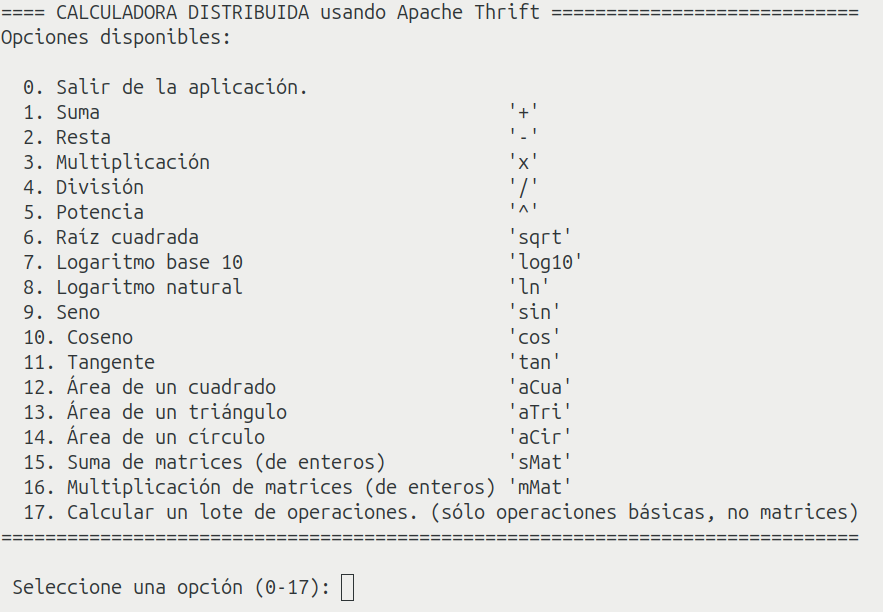
\includegraphics[width=1\linewidth]{./imagenes_necesarias/menu_calculadora.png}
				\caption{Menú de opciones de la calculadora.}
				\label{fig:menu_calculadora}
			\end{figure}
			
			En él se puede ver la gran cantidad y variedad de operaciones matemáticas que hay disponibles. Si introducimos 0 (\texttt{opcion = 0}), saldremos de la aplicación. En otro caso, tras realizar la operación seleccionada con  anterioridad, nos seguirá apareciendo el menú constantemente, por si queremos realizar más de una operación. 
			
			Además, tras realizar la operación se nos mostrará un mensaje diciendo \texttt{Pulse 'Enter' para continuar...}, y si lo pulsamos, nos volverá a aparecer el menú para volver a elegir otra operación. El motivo de hacerlo así es para no sobrecargar la interfaz o mejor dicho, la terminal, y que el usuario que utilice la calculadora no se sienta abrumado.
			
			\subsubsection{Ejemplo nº1. Operación básica. División}
				En este ejemplo vamos a realizar una división, vamos a dividir $44/35$. Para ello seguimos los siguientes pasos:
				\begin{enumerate}
					\item 	Introducimos la opción nº 4 \texttt{opcion = 4}.
					\item Después introducimos el primer operando (dividendo) $44$ y pulsamos \texttt{'Enter'}.
					\item A continuación introducimos el segundo operando (divisor) $35$ y volvemos a pulsar \texttt{'Enter'}. Como vemos, se nos mostrará el resultado por pantalla. 
					\item  Finalmente volvemos a pulsar \texttt{'Enter'} para que nos vuelva a aparecer el menú y poder continuar.
				\end{enumerate}
			
				\begin{figure}[H]
					\centering
					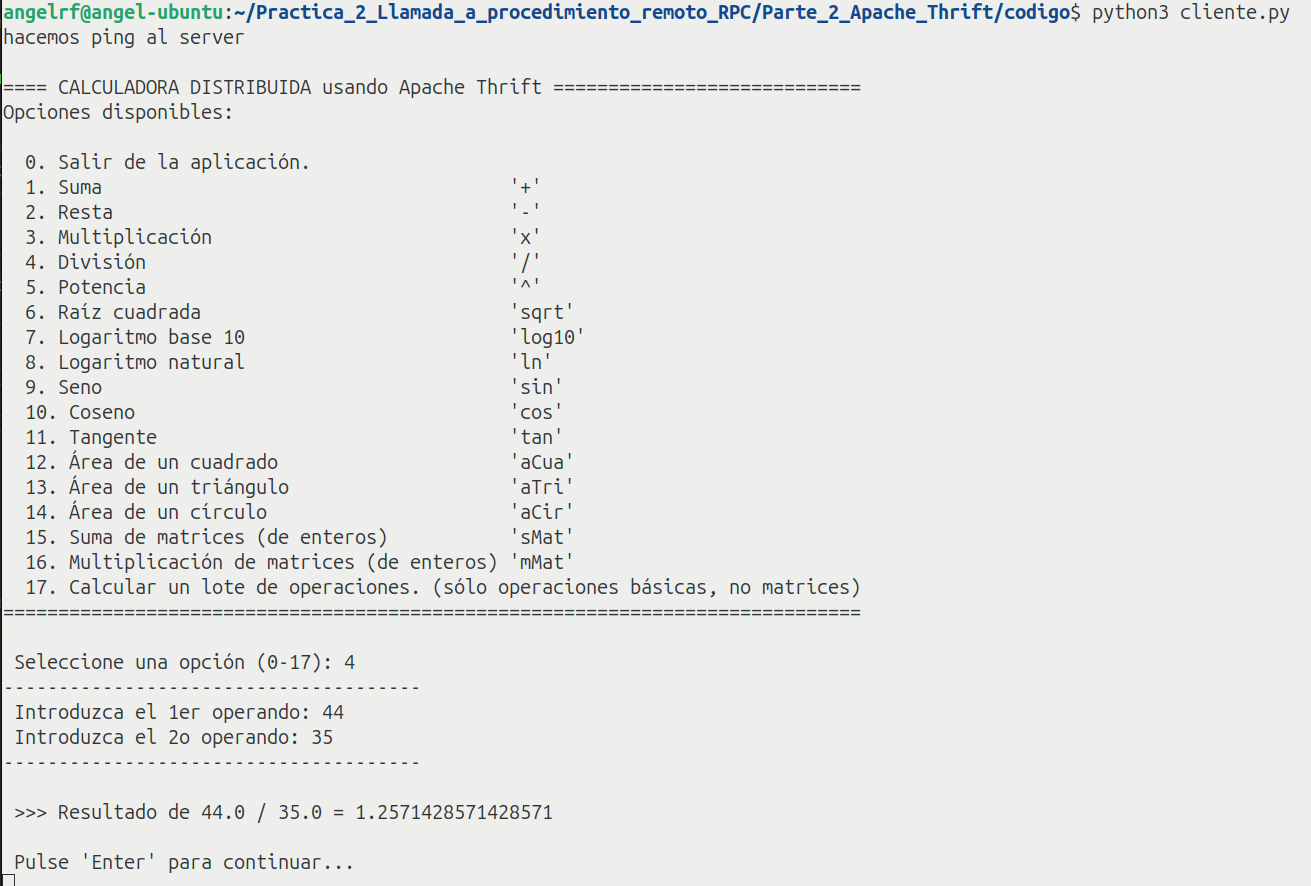
\includegraphics[width=0.8\linewidth]{./imagenes_necesarias/ejemplo1_nro1_division_cliente.png}
					\caption{Ejemplo nº1. Dividir 44 entre 35, visto desde el lado del cliente.}
					\label{fig:ejemplo1_nro1_division_cliente}
				\end{figure}
				
				En la siguiente imagen vemos un ejemplo de la excepción que se puede generar al intentar realizar una operación que no es válida, como por ejemplo, dividir entre 0.
				
				\begin{figure}[H]
					\centering
					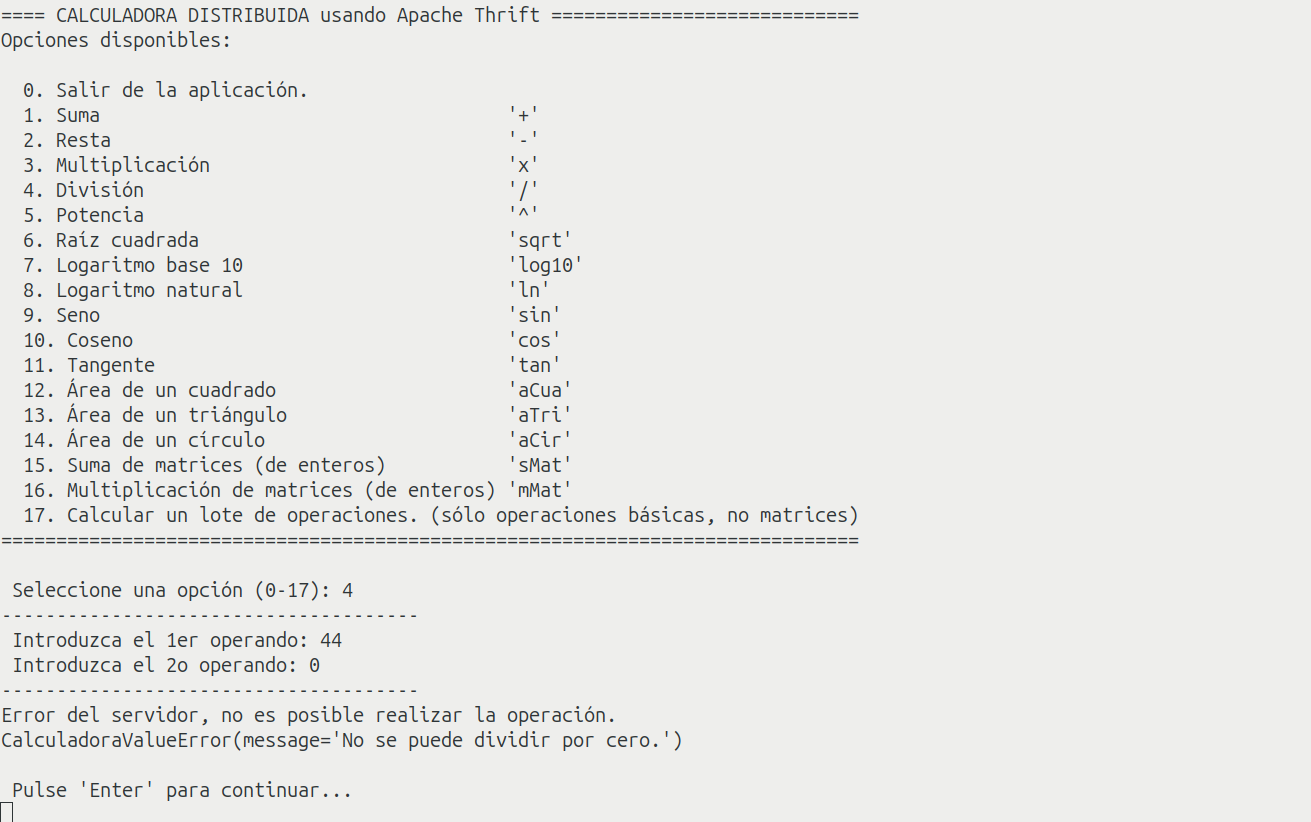
\includegraphics[width=0.8\linewidth]{./imagenes_necesarias/ejemplo2_nro1_division_cliente.png}
					\caption{Ejemplo nº1. Error al intentar dividir 44 entre 0, visto desde el lado del cliente.}
					\label{fig:ejemplo2_nro1_division_cliente}
				\end{figure}
				
				Desde el lado del servidor (esta vez he ejecutado el servidor implementado en Python), se vería así:
				
				\begin{figure}[H]
					\centering
					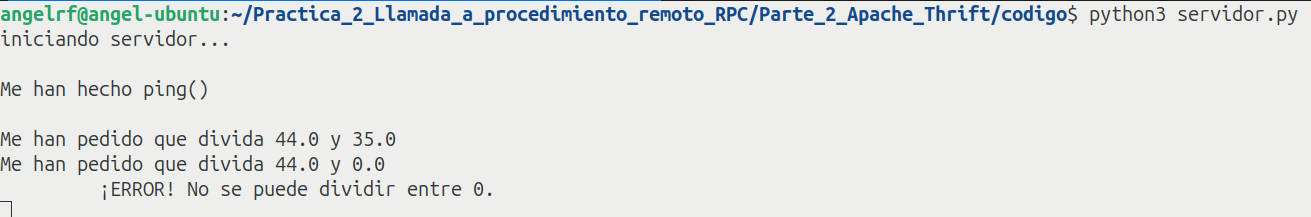
\includegraphics[width=1\linewidth]{./imagenes_necesarias/ejemplo_nro1_division_servidor.png}
					\caption{Ejemplo nº1 visto desde el lado del servidor.}
					\label{fig:ejemplo_nro1_division_servidor}
				\end{figure}
				
			
			\subsubsection{Ejemplo nº2. Operación básica. Área de un Círculo.}	
				En este ejemplo vamos a calcular el área de un triángulo con \texttt{base = 12.5} y \texttt{altura = 15.3} Para ello seguimos los siguientes pasos:
				\begin{enumerate}
					\item Introducimos la opción nº 13 \texttt{opcion = 13}.
					\item Después introducimos la base del triángulo: $12.5$ y pulsamos \texttt{'Enter'}.
					\item A continuación introducimosla altura del triángulo: $15.3$ y volvemos a pulsar \texttt{'Enter'}. Como vemos, se nos mostrará el resultado por pantalla. 
					\item  Finalmente volvemos a pulsar \texttt{'Enter'} para que nos vuelva a aparecer el menú y poder continuar.
				\end{enumerate}
				
				\begin{figure}[H]
					\centering
					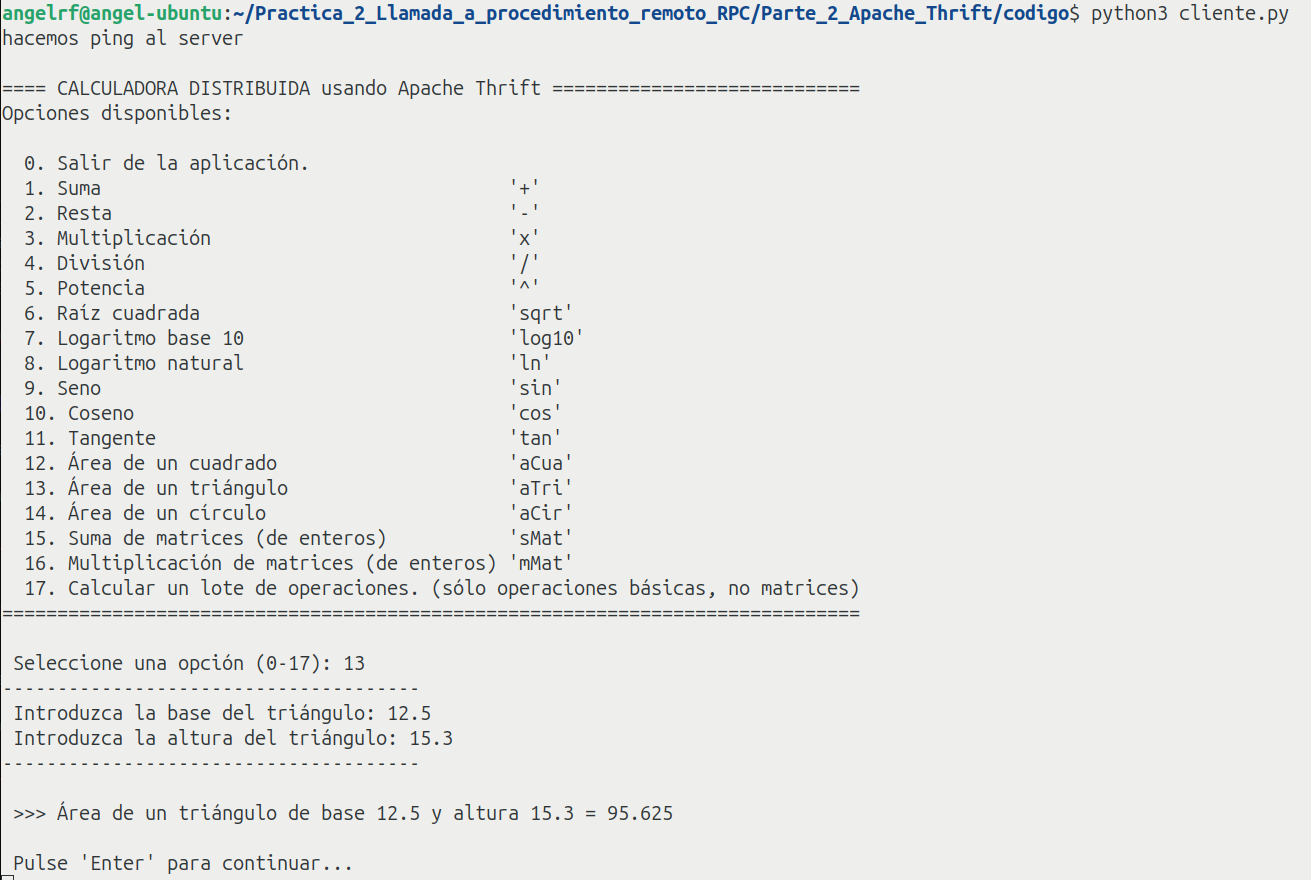
\includegraphics[width=1\linewidth]{./imagenes_necesarias/ejemplo_nro2_cliente.png}
					\caption{Ejemplo nº2. Área de un Triángulo visto desde el lado del cliente.}
					\label{fig:ejemplo_nro2_cliente}
				\end{figure}
				
				Desde el lado del servidor (esta vez he ejecutado el servidor implementado en Java), se vería así:
				
				\begin{figure}[H]
					\centering
					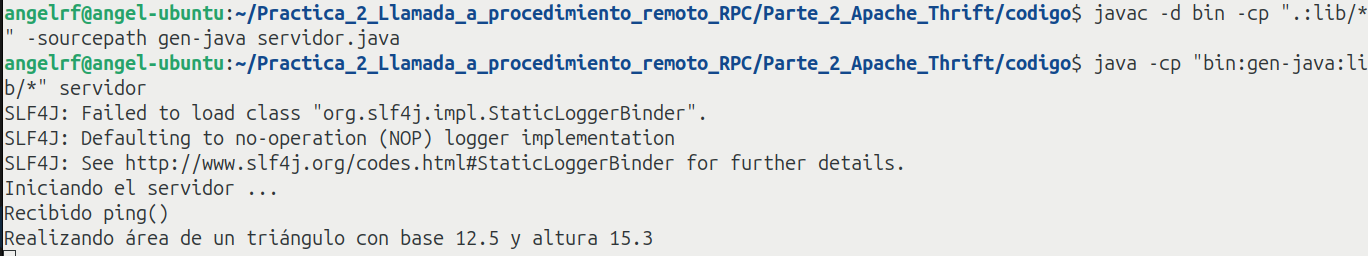
\includegraphics[width=1\linewidth]{./imagenes_necesarias/ejemplo_nro2_servidor.png}
					\caption{Ejemplo nº2 visto desde el lado del servidor.}
					\label{fig:ejemplo_nro2_servidor}
				\end{figure}
				
				\newpage
			
			\subsubsection{Ejemplo nº3. Operación con matrices}
				En este ejemplo vamos a calcular la \textbf{suma de dos matrices} de dimensiones \texttt{2 x 3}. Los pasos a seguir son:
				\begin{enumerate}
					\item Introducimos la opción nº 15 \texttt{opcion = 15}.
					\item Introducimos el número de filas de la 1ª matriz.
					\item Después el número de columnas de la 1ª matriz.
					\item A continuación introducimos la primera fila de la 1ª matriz, \textbf{los elementos tienen que ir separados por un espacio}. Al terminar pulsamos\texttt{'Enter'}. 
					\item Repetimos la misma operación anterior para la segunda fila de la 1ª matriz. Al terminar pulsamos\texttt{'Enter'} y se nos mostrará como ha quedado la 1ª matriz.
					\item Introducimos el número de filas de la 2ª matriz. (Debe ser el mismo que el de la 1ª matriz)
					\item Después el número de columnas de la 2ª matriz. (Debe ser el mismo que el de la 1ª matriz)
					\item Ahora introducimos la primera fila de la 2ª matriz, los elementos tienen que ir separados por un espacio. Al terminar pulsamos\texttt{'Enter'}. 
					\item Repetimos la misma operación anterior para la segunda fila de la 2ª matriz,los elementos tienen que ir separados por un espacio. Al terminar pulsamos\texttt{'Enter'} y se nos mostrará como ha quedado la 2ª matriz.		
					\item Nos aparecerá la matriz resultado de realizar la operación.			
					\item  Finalmente volvemos a pulsar \texttt{'Enter'} para que nos vuelva a aparecer el menú y poder continuar.
				\end{enumerate}
				
				\begin{figure}[H]
					\centering
					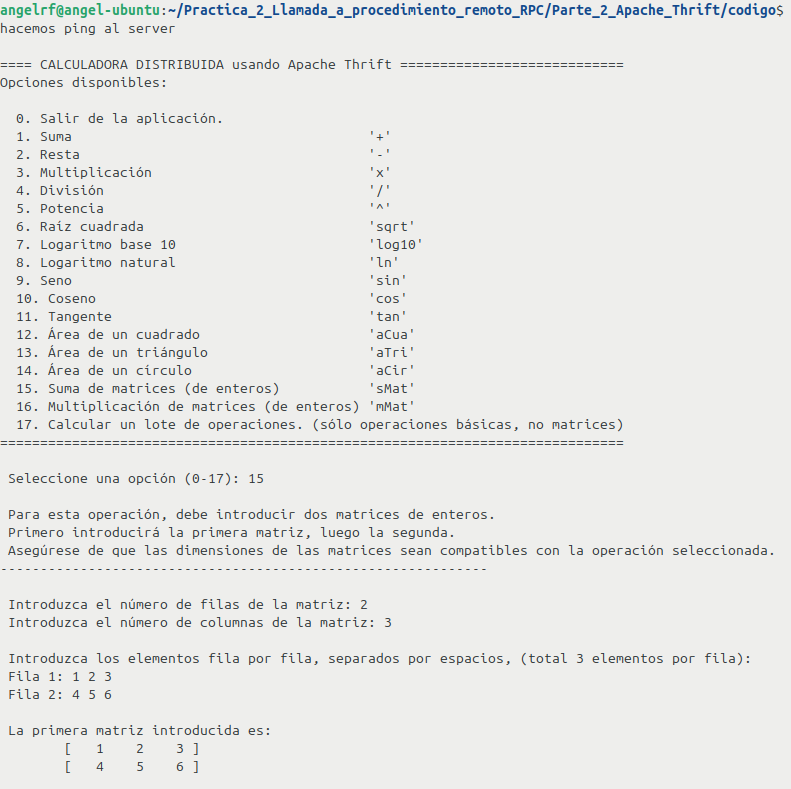
\includegraphics[width=0.7\linewidth]{./imagenes_necesarias/ejemplo_nro3_suma_cliente_1-2.png}
					\caption{Imagen 1/2. Ejemplo nº3. Suma de matrices visto desde el lado del cliente.}
					\label{fig:ejemplo_nro3_cliente_1-2}
				\end{figure}
				
				\begin{figure}[H]
					\centering
					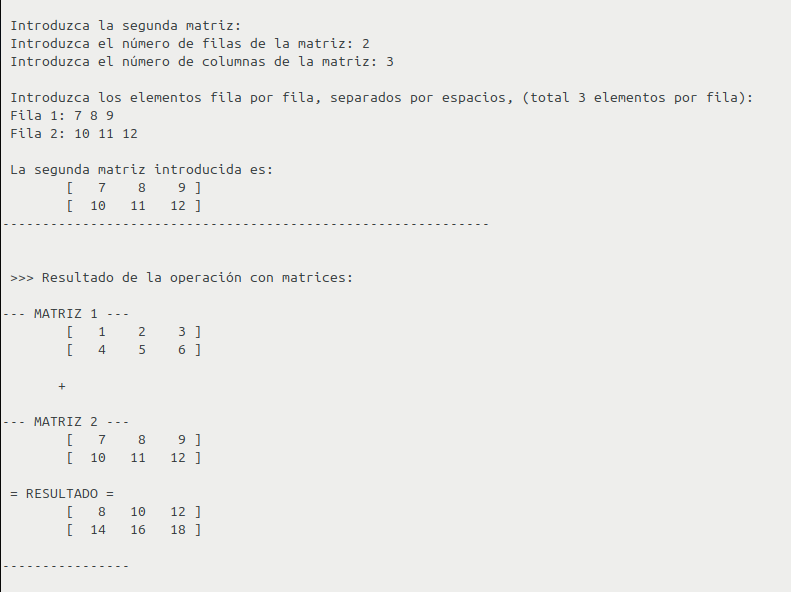
\includegraphics[width=0.7\linewidth]{./imagenes_necesarias/ejemplo_nro3_suma_cliente_2-2.png}
					\caption{Imagen 2/2. Ejemplo nº3. Suma de matrices visto desde el lado del cliente.}
					\label{fig:ejemplo_nro3_cliente_2-2}
				\end{figure}
				
				Desde el lado del servidor, se vería así:
				
				\begin{figure}[H]
					\centering
					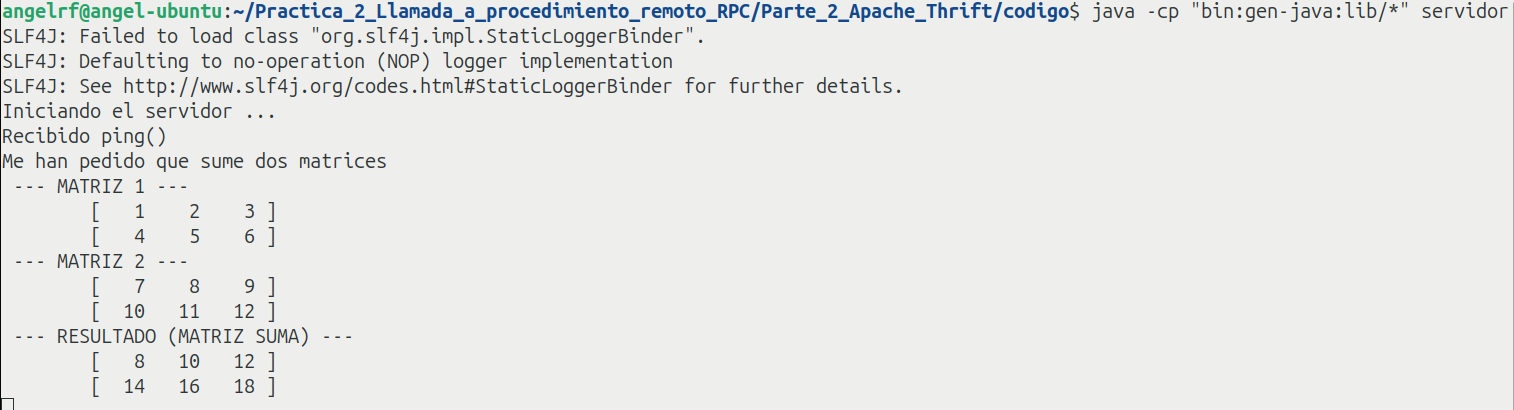
\includegraphics[width=1\linewidth]{./imagenes_necesarias/ejemplo_nro3_suma_servidor.png}
					\caption{Ejemplo nº3. Suma de matrices visto desde el lado del servidor.}
					\label{fig:ejemplo_nro3_servidor}
				\end{figure}
			
			\subsubsection{Ejemplo nº4. Procesamiento de un lote de operaciones}.
				En este ejemplo vamos a calcular  \textbf{un lote de 3 operaciones}. Los pasos a seguir son:
				\begin{enumerate}
					\item Introducimos la opción nº 17 \texttt{opcion = 17}.
					\item Introducimos el número de operaciones que queremos realizar: \texttt{3} y pulsamos\texttt{'Enter'}.
					\item Introducimos el operador de la 1ª operación. En este caso se trata de una raíz cuadrada: \texttt{sqrt}. Volvemos a pulsar\texttt{'Enter'}.
					\item A continuación introducimos el primer operando (en este caso sería el radicando). Al terminar pulsamos\texttt{'Enter'}. 
					\item Repetimos los pasos nº3 y nº4 para la 2ª operación, que es el área de un cuadrado de lados \texttt{5.9}. Sería el operador \texttt{aCua}.
					\item Repetimos los pasos nº3 y nº4 para la 3ª operación, que es el seno de \texttt{90} grados. Sería el operador \texttt{sin}.
					\item A continuación nos aparecerán los resultados de todas las operaciones.
					\item  Finalmente volvemos a pulsar \texttt{'Enter'} para que nos vuelva a aparecer el menú y poder continuar.
				\end{enumerate}
				
				\begin{figure}[H]
					\centering
					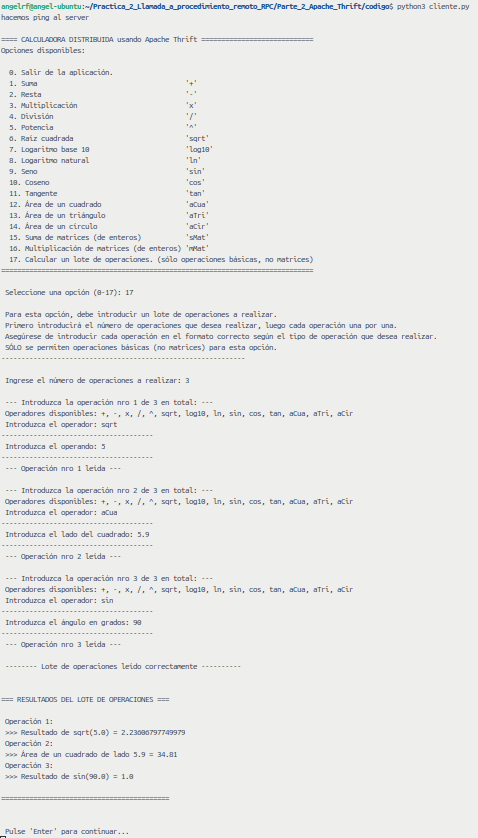
\includegraphics[width=0.9\linewidth]{./imagenes_necesarias/ejemplo_nro4_cliente.png}
					\caption{Ejemplo nº4. Lote de operaciones visto desde el lado del cliente.}
					\label{fig:ejemplo_nro4_cliente}
				\end{figure}
				
				Desde el lado del servidor, se vería así:
				
				\begin{figure}[H]
					\centering
					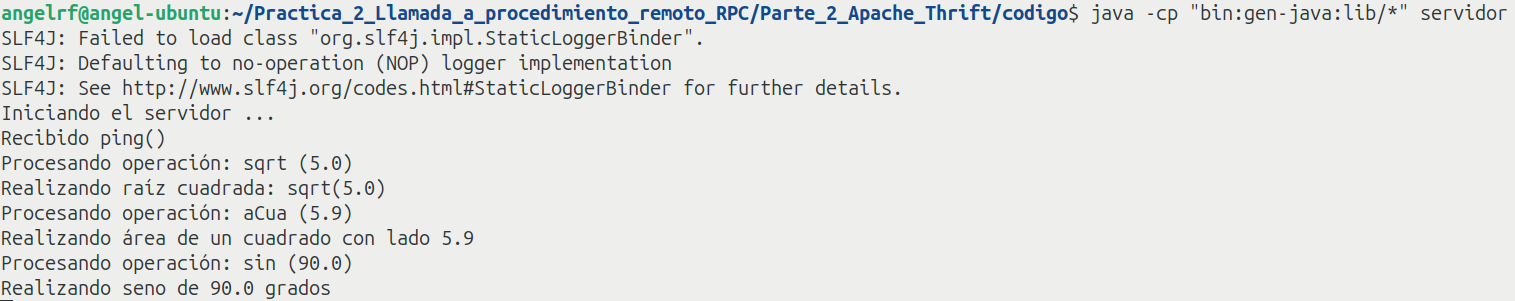
\includegraphics[width=1\linewidth]{./imagenes_necesarias/ejemplo_nro4_servidor.png}
					\caption{Ejemplo nº4. Lote de operaciones visto desde el lado del servidor.}
					\label{fig:ejemplo_nro4_servidor}
				\end{figure}

\end{document}